\documentclass[a4paper,norsk]{article}
\usepackage[latin1]{inputenc}
\usepackage[T1]{fontenc}
\usepackage{babel,textcomp,listings, subfigure,graphicx}
                                    
\title{Mandatory assignment 2, MEK4300}
\author{Sebastian Gjertsen}
\begin{document}
\maketitle
\section*{i}
\subsection*{a)}
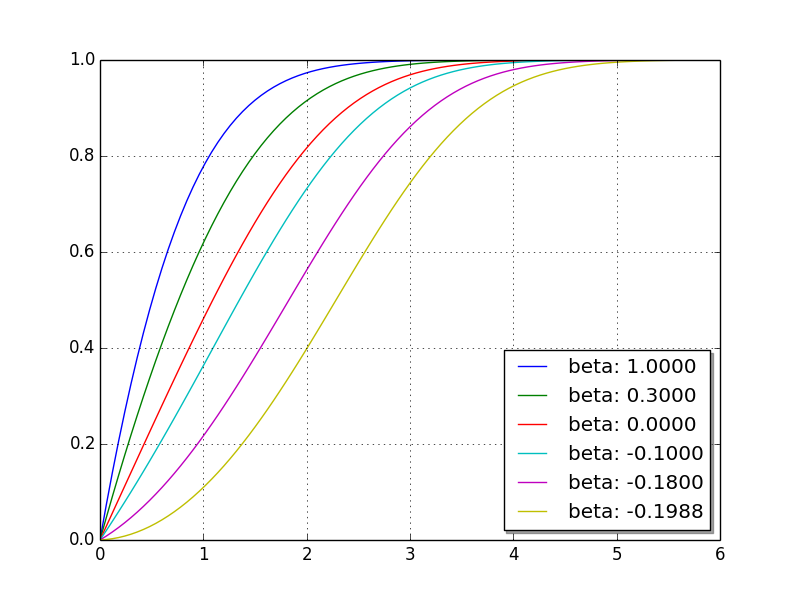
\includegraphics[trim = 0mm 0mm 0mm 0mm, clip, scale=0.3]{f_derivative.png} 
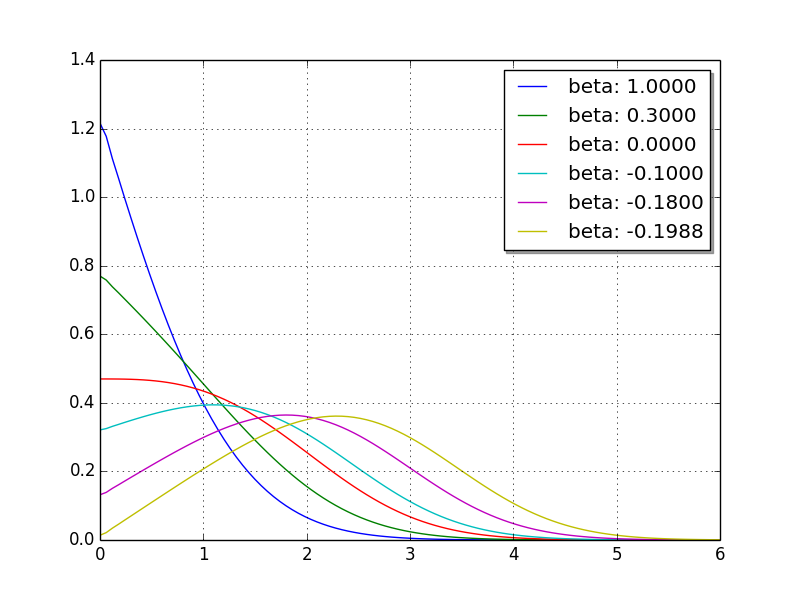
\includegraphics[trim = 0mm 0mm 0mm 0mm, clip, scale=0.3]{f_double_derivative.png} 
In the first section I have reproduced figure 4-11 in White, with different $beta$ values


\subsection*{b)}
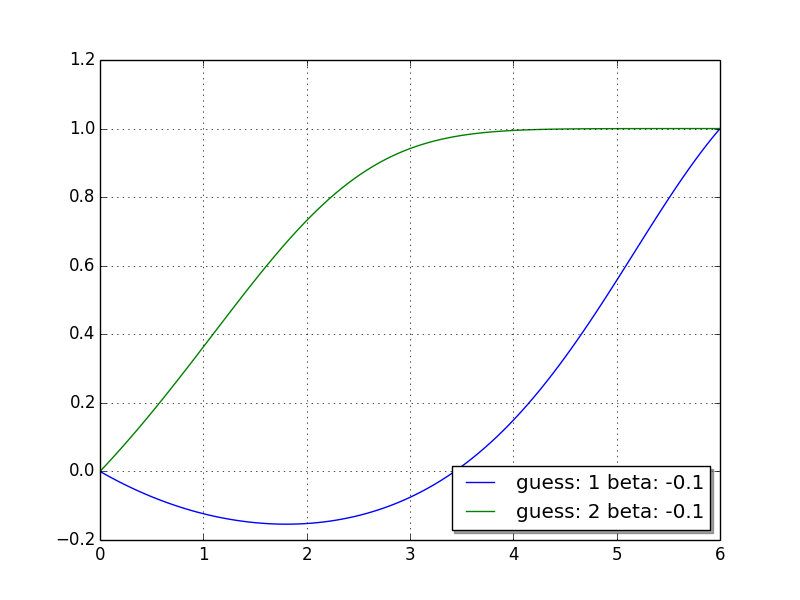
\includegraphics[trim = 0mm 0mm 0mm 0mm, clip, scale=0.3]{guess.png} 
The two guesses in the plots are with (0,0) and (1,1)

\section*{ii}
\subsection*{a)}
In the first test with steady solver and Re = 20
$$C_D= 5.79392133271, C_L = 0.00871442276844, \Delta P = 0.11435196$$
which is pretty close compare to the benchmark :$$C_D =  5.5567 , C_L = 0.0106 , \Delta P =  0.1172 $$
\subsection*{b)}
Using $dt = 0.0005 $ and a mesh with:  5713 vertices 11433 elements


\end{document}
